\section{experimental evaluation}\label{sec:exp}
In this section, we conduct extensive experiments by comparing the proposed hash table designs with several state-of-the-art approaches for GPU-based hash tables. 
We will introduce the experimental setup and the discuss the results. 

\subsection{Experiment Setup}\label{sec:exp:setup}

\vspace{1mm}\noindent\textbf{Baselines.} We compare the proposed approach in this paper with several state-of-the-art hash table implementations on GPUs and CPUs. 
\begin{itemize}
	\item \cudpp is a popular CUDA primitive library\footnote{https://github.com/cudpp/cudpp} which contains the cuckoo hash table implementation published in~\cite{alcantara2009real}. 
	\cudpp employs four hashing functions and each hash value stores only one KV pair with 64 bits size (32 bits for key and 32 bits for value). 
	\cudpp only supports \formal{insert} and \formal{find} operations. 
	\item \megakv is a state-of-the-art approach for GPU-based key value store published in~\cite{zhang2015mega}. It employs a cuckoo hash with two hash functions.
	\megakv also allocates a bucket for each hash value. However, it does not lock a bucket when performing update. Instead, it uses intra-block synchronization to resolve race condition. 
	\item \linear is a GPU-based hash table which uses linear open addressing to resolve conflicts \cite{hong2010mapcg}. 
	\item \google is an efficient CPU-based hash table implementation\footnote{https://github.com/sparsehash/sparsehash-c11/}. We choose the \emph{dense\_hash\_map} implementation since it provides the best efficiency.
	\item \voter is the approach proposed in this paper.
\end{itemize}
We adopt the original implementations of \cudpp and from their corresponding inventors. 
For \megakv, we note that its intra-block synchronization could lead to inconsistency issue as well as a large number of insertion failures, especially when the filled factor is high.  
Thus, we revise its code by replacing the intra-block synchronization with atomicExch to resolve the race condition. The adoption of atomicExch preserves the design principle of \megakv for \emph{not} locking the entire bucket for updates. Moreover, it leads to less insertion failures and similar performance against its original implementation. 
For \linear, we implement the CUDA version of the algorithm proposed in \cite{hong2010mapcg}.

Note that we do not compare with the dynamic GPU hash approach proposed in \cite{ashkiani2018dynamic} for two major reasons. First, we cannot obtain the original implementation from its authors. Second, the approach devises a dedicated memory allocator other than cudaMalloc. A dedicated allocator will improve the performance but add complexity to the system. Additionally, it needs to occupy a large memory in advance and is not transparent to other GPU applications.
In contrast, our proposed approach only use native allocator supported. 
We do not compare with \cite{breslow2016horton} since it only improves \megakv marginally using a more costly insertion process.

\begin{table}[t]
	\caption{The datasets used in the experiments.}
	\label{table:exp_data_sets}
	\centering
	\begin{tabular}{|c|c|c|c|}
		\hline
		Datasets & KV pairs & Unique keys & Max Duplicates \\ \hline
		\dstwitter &50,876,784 & 44,523,684&4\\ \hline
		\dsreddit & 48,104,875 & 41,466,682 &2 \\ \hline
		\dstpch &50,000,000 & 45,159,880&4\\ \hline
		\dsali &10,000,000 & 4,583,941&14\\ \hline
		\dsrandom & 100,000,000& 100,000,000& 1 \\ \hline
	\end{tabular}
\end{table}

\vspace{1mm}\noindent\textbf{Datasets.} We evaluate all compared approaches using several real world and synthetic datasets described as follows:
\begin{itemize}
	\item \dstwitter: Twitter is an online social network where users perform actions include \emph{tweet}, \emph{retweet}, \emph{quote} and \emph{reply}.
	We crawl these actions for one week via Twitter stream API\footnote{https://dev.twitter.com/streaming/overview} on trending topics US president election, 2016 NBA finals and Euro 2016. The dataset contains 50,876,784 KV pairs.
	\item \dsreddit: Reddit is an online forum where users perform actions include \emph{post} and \emph{comment}. We collect all Reddit \emph{comment} actions in May 2015 from \emph{kaggle}\footnote{https://www.kaggle.com.reddit/reddit-comments-may-2015} and query the Reddit API for the \emph{post} actions the same period. The dataset contains 48,104,875 actions as KV pairs. 
 	\item \dstpch: Lineitem is a synthetic table generated by the TPC-H benchmark\footnote{https://github.com/electrum/tpch-dbgen}. We generate  100,000,000 rows of the lineitem table and combine the \emph{orderkey},\emph{linenumber} and \emph{partkey} column as keys. 
	\item \dsrandom: Random is a synthetic dataset generated from a normal distribution. We have deduplicated the data and generate 100,000,000 KV pairs.  
	\item \dsali: Databank is a PB-scale data warehouse that stores user behavior data in past one year of Alibaba's economic entity. Due to confidentially, we sample 10,000,000 transactions and the dataset contains 4,583,941 unique data ids as keys.
\end{itemize}
The summary of the datasets can be found in Table~\ref{table:exp_data_sets}.
Since all GPU approaches (except for \voter) only supports 32 bit key and 32 bit value, we hash longer keys to 32 bits and truncate all values to 32 bits across all datasets. 


\begin{table}
	\centering
	\caption{Parameters in the experiments}
	\label{tbl:parameters}
	\begin{tabular}{|c|c|c|}
		\hline
		\textbf{Parameter} & \textbf{Settings} & \textbf{Default} \\ \hline
		$\alpha$ & 25\%, 30\%, 35\%, 40\%, 45\% & 40\% \\ \hline
		$\beta$  & 75\%, 80\%, 85\%, 90\%, 95\% & 90\% \\ \hline
		$r$ & 0.1, 0.2, 0.3, 0.4, 0.5 & 0.4 \\ \hline
	\end{tabular}
\end{table}



\vspace{1mm}\noindent\textbf{Static Hashing Comparison (Section~\ref{sec:exp:static}).}
Under the static setting, we evaluate \formal{insert} and \formal{find} performance among all compared approaches. 
In particular, we insert all KV pairs from the datasets followed by issuing 1 million random search queries. 
The intention for testing the static setting is to see if \voter can produce competitive performance, even though it uses a slightly inefficient atomicCAS (compared with atomicExch used by the GPU baselines) to lock a bucket for supporting KV pairs with larger size.  

\vspace{1mm}\noindent\textbf{Dynamic Hashing Comparison (Section~\ref{sec:exp:dynamic}).}
Under the dynamic setting, we generate the workloads by batching the hash table operations. 
We partition the datasets into batches of $1$ million insertions. 
For each batch, we augment $1$ million \formal{find} operations and $1 \cdot r$ million \formal{delete} operations,
where $r$ is a parameter to balance insertions and deletions.
After we exhaust all the batches obtained from the datasets, we rerun these batches by swapping the \formal{insert} and \formal{delete} operations in any batch. 
We evaluate the performance of all compared approaches except \cudpp as it does not support deletions. 
Since all approaches other than \voter are static hash tables, we double/half the memory usage followed by rehashing all KV pairs as their resizing strategy, if the corresponding filled factor falls out of the specified range. 
Moreover, if an insertion failure is found for a compared approach, we trigger its resizing strategy.

\begin{figure*}[t]
	\begin{minipage}{0.3\linewidth}\centering
		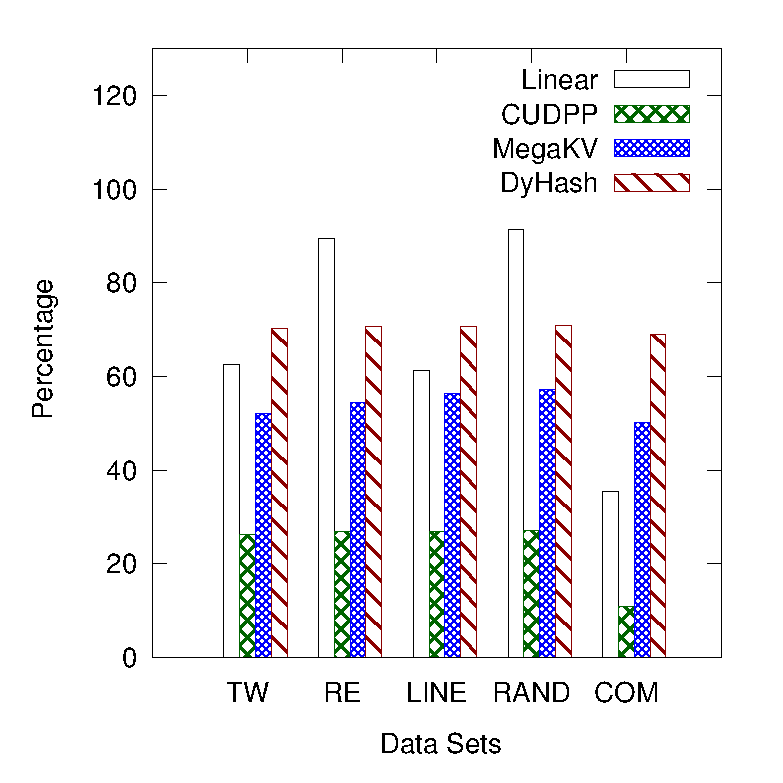
\includegraphics[width=\linewidth]{pic/static-profi/warp.eps}
		\centerline{Warp Efficiency}
	\end{minipage}
	\hfill
	\begin{minipage}{0.3\linewidth}\centering
		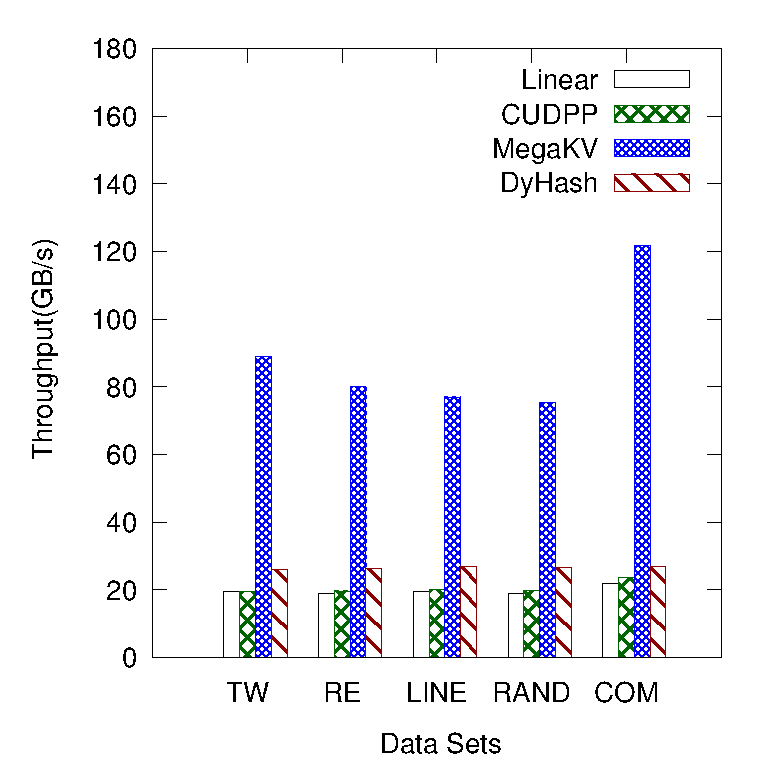
\includegraphics[width=\linewidth]{pic/static-profi/L2-read.eps}
		\centerline{Cache Utilization}
	\end{minipage}
	\hfill
	\begin{minipage}{0.3\linewidth}\centering
		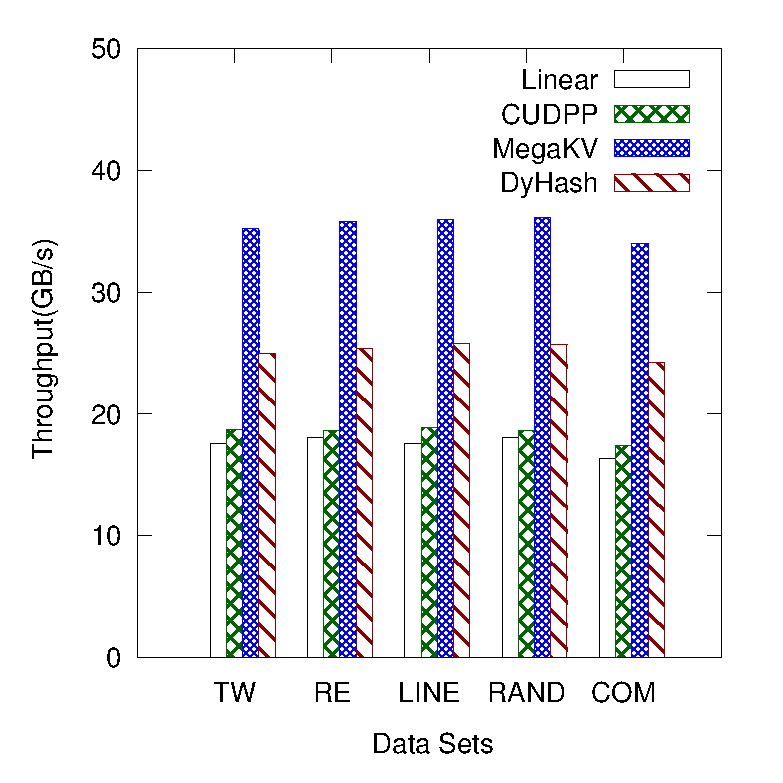
\includegraphics[width=\linewidth]{pic/static-profi/memory-read.eps}
		\centerline{Memory Bandwidth Utilization}
	\end{minipage}
	\caption{GPU profiling results for static hashing comparison.}
	\label{fig:static:profile}
\end{figure*}

\vspace{1mm}\noindent\textbf{Parameters.}
We vary the parameters when comparing \voter with the baselines.
$\alpha$ is the lower bound on the filled factor $\theta$ for all compared approaches,
whereas $\beta$ is the respective upper bound.
$r$ is the ratio of insertions over deletions in a processing batch. 
The settings of the aforementioned parameters could be found in Table~\ref{tbl:parameters}.

\vspace{1mm}\noindent\textbf{Experiment Environment.}
We conduct the experiments on an Intel Xeon E5-2620 Server equipped with NVIDIA GeForce GTX 1080.The GTX 1080 is built on Pascal architecture with 20 SMs and 128 SPs per SM. The GTX 1080 has 8 GB of GDDR5 memory. Evaluations are performed using CUDA 8.0 on Ubuntu 16.04.3. The optimization level (-O3) is applied for compiling all programs.



\begin{figure}[t!]
	\begin{minipage}{0.48\linewidth}\centering
		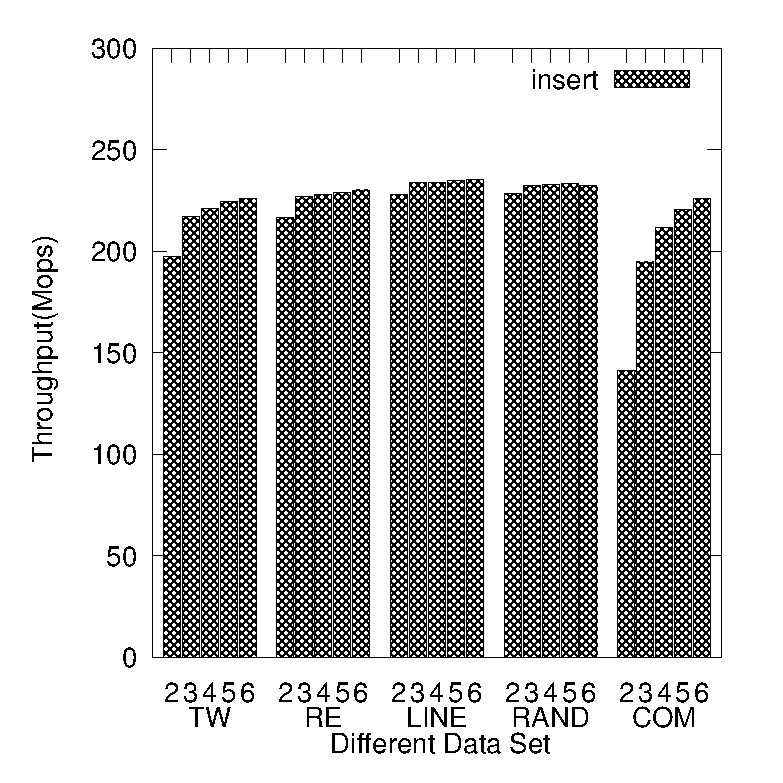
\includegraphics[width=\linewidth]{pic/tunning/tunning-insert.eps}
		\centerline{\formal{insert}}
	\end{minipage}
	\hfill
	\begin{minipage}{0.48\linewidth}\centering
		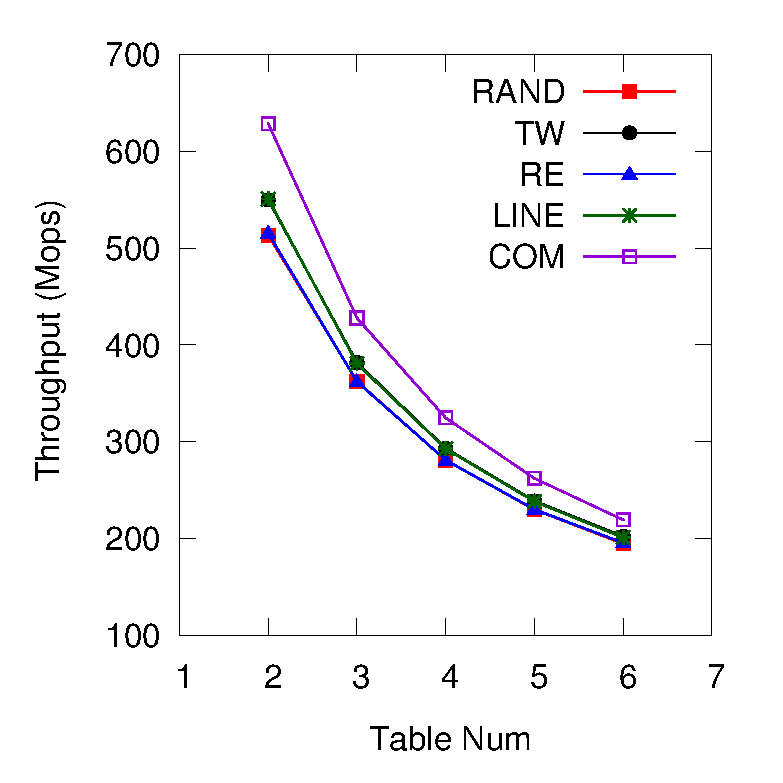
\includegraphics[width=\linewidth]{pic/tunning/tunning-search.eps}
		\centerline{\formal{find}}
	\end{minipage}
	\caption{Throughput of \voter when varying the number of hash tables.}
	\label{fig:vary-table}
\end{figure}


\subsection{Tunning Parameters}

A key parameter that affects the performance of \voter is the number of hash table chosen. For the static scenario, we present the throughput performance of \formal{insert} and \formal{find} for varying number of hash tables in Figure~\ref{fig:vary-table}, while fixing the memory space of the entire structure to ensure the default filled factor. 
The throughput of \formal{insert} increases with more hash tables, since there are more alternative locations for inserting a KV pair. However, the marginal improvement drops for a larger number of hash tables. The throughput of \formal{find} falls with more hash tables as additional locations need to be scanned to locate a KV pair. Thus, one can tradeoff the performance between \formal{insert} and \formal{find} operations by varying the number of tables. In this paper, we choose three hash tables as our default implementation as it provides the best balance. 


\begin{figure}[t!]
	\begin{minipage}{0.48\linewidth}\centering
		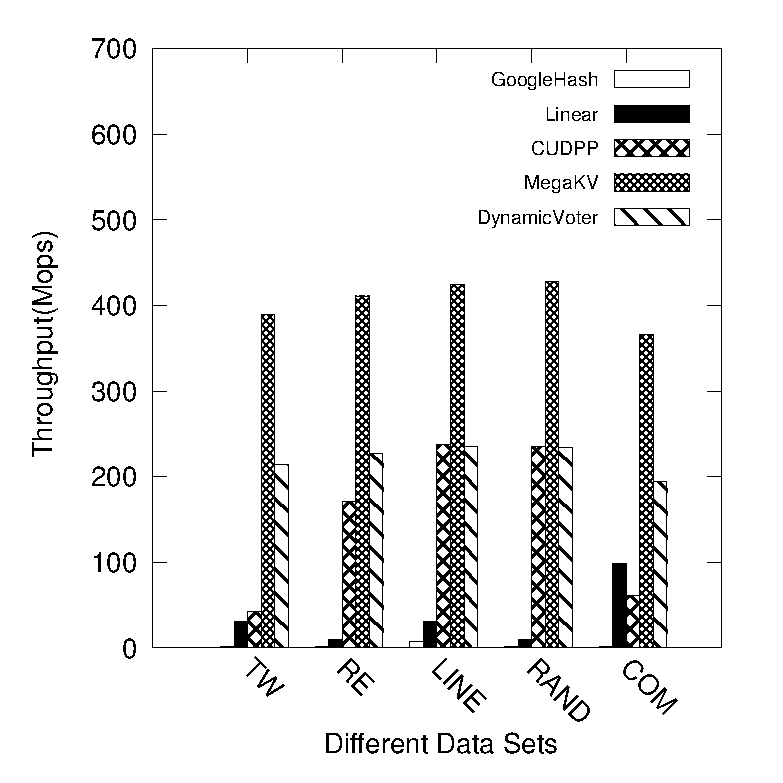
\includegraphics[width=\linewidth]{pic/static/static_insert.eps}
		\centerline{\formal{insert}}
	\end{minipage}
	\hfill
	\begin{minipage}{0.48\linewidth}\centering
		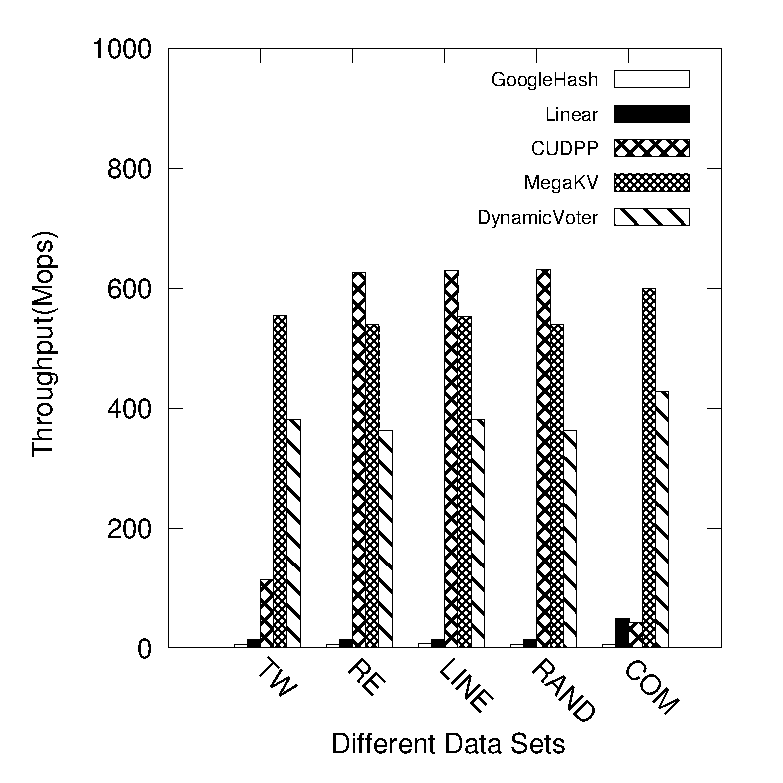
\includegraphics[width=\linewidth]{pic/static/static_search.eps}
		\centerline{\formal{find}}
	\end{minipage}
	\caption{Throughput of all compared approaches under the static setting.}
	\label{fig:static}
\end{figure}

\begin{figure*}[ht]
	\begin{minipage}{0.19\linewidth}\centering
		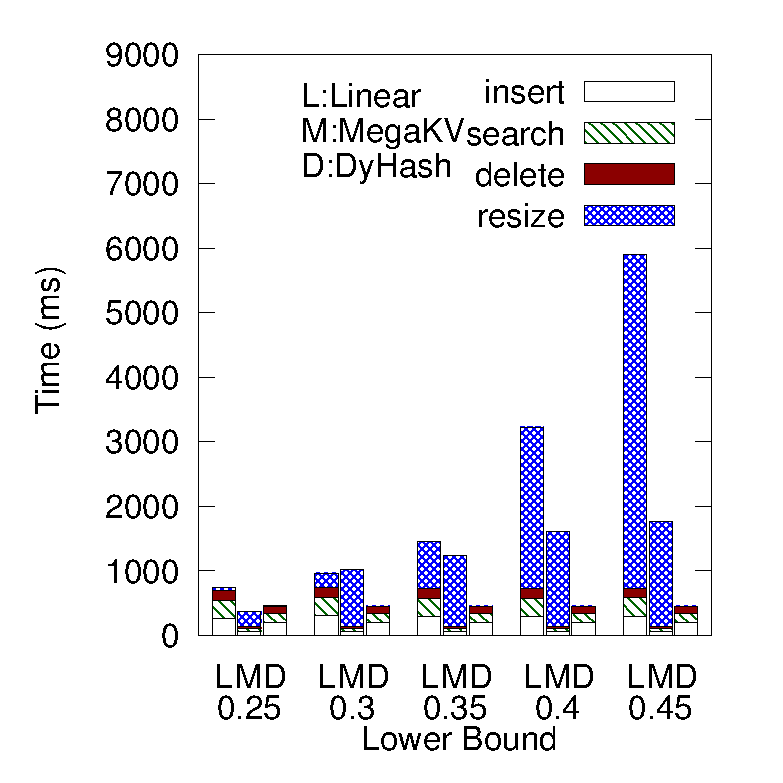
\includegraphics[width=\linewidth]{pic/dynamic/twitter/diff_lower.eps}
		\centerline{\dstwitter}
	\end{minipage}
	\begin{minipage}{0.19\linewidth}\centering
		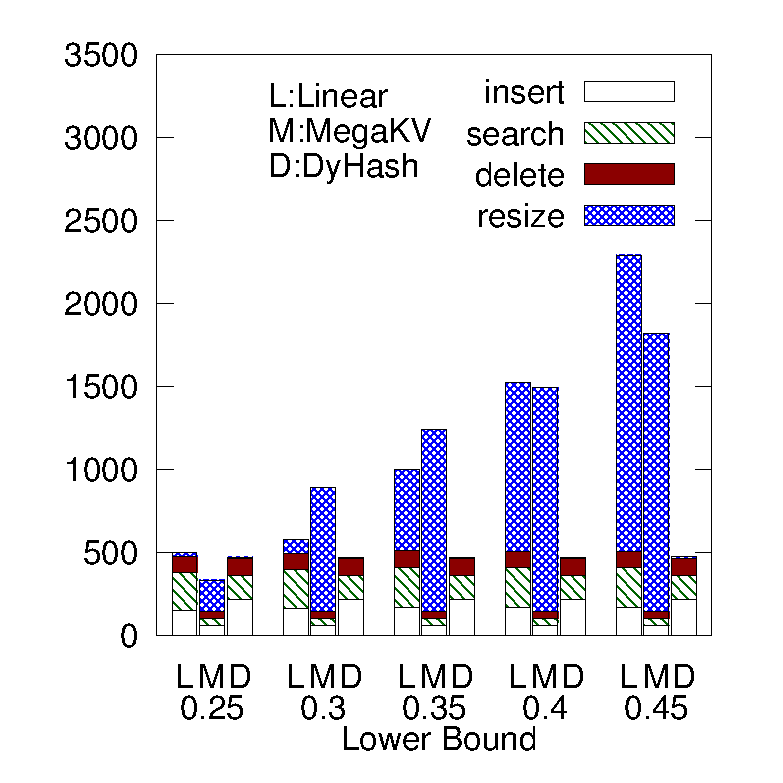
\includegraphics[width=\linewidth]{pic/dynamic/reddit/diff_lower.eps}
		\centerline{\dsreddit}
	\end{minipage}
	\begin{minipage}{0.19\linewidth}\centering
		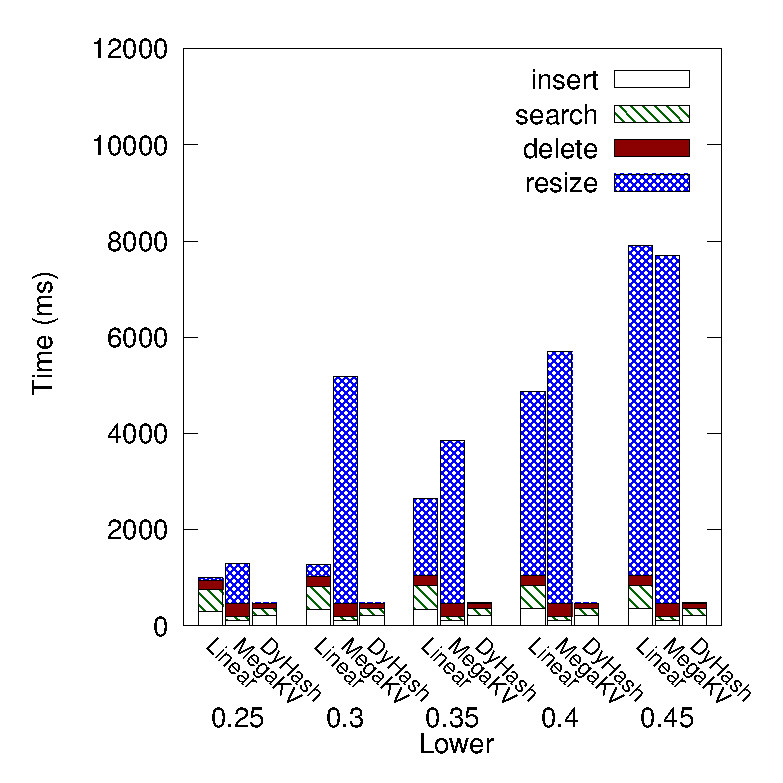
\includegraphics[width=\linewidth]{pic/dynamic/tpch/diff_lower.eps}
		\centerline{\dstpch}
	\end{minipage}
	\begin{minipage}{0.19\linewidth}\centering
		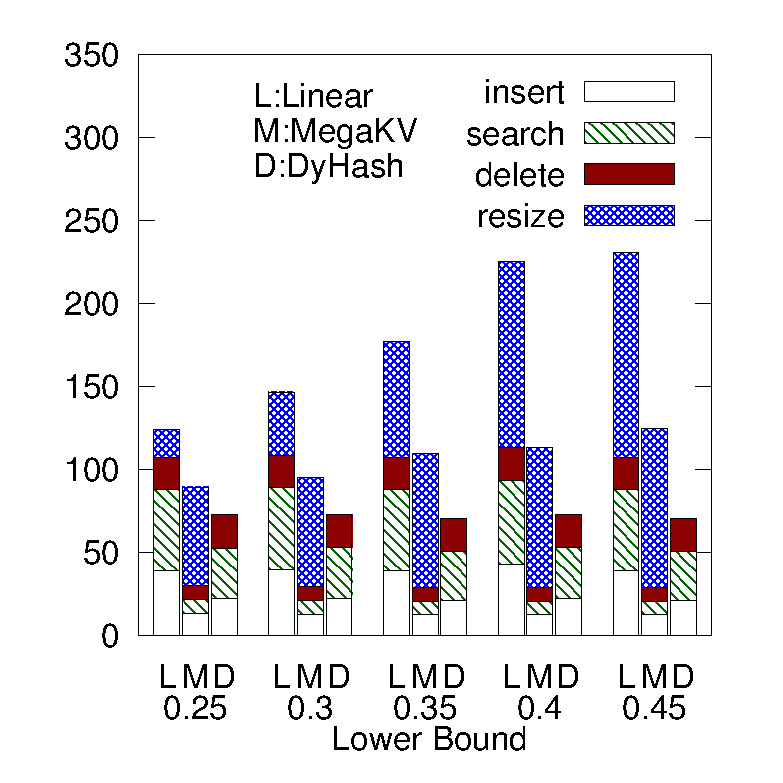
\includegraphics[width=\linewidth]{pic/dynamic/ali/diff_lower.eps}
		\centerline{\dsali}
	\end{minipage}
	\begin{minipage}{0.19\linewidth}\centering
		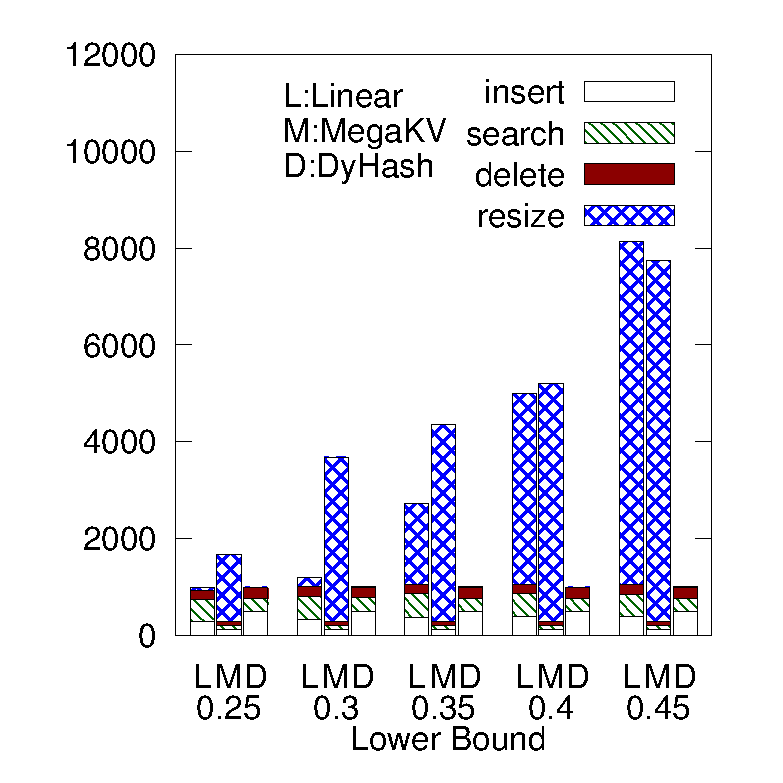
\includegraphics[width=\linewidth]{pic/dynamic/random/diff_lower.eps}
		\centerline{\dsrandom}
	\end{minipage}
	\caption{Run time for varying $\alpha$.}
	\label{fig:vary-alpha-time}
\end{figure*}
\begin{table*}[ht]\centering
	\begin{minipage}{0.45\linewidth}\centering
		\caption{The failure of TW (Percentages).}
		\begin{tabular}{|c|c|c|c|c|c|}
			\hline
			& 0.75 & 0.8 & 0.85 & 0.9 & 0.95\\ \hline
			Linear &0.0 & 0.0 &4.6e-5  & 1.1e-3 & 3.9e-1 \\ \hline
			CUDPP & 0.0 & 0.0 &0.0  & 0.0 & 3.8e-5 \\ \hline
			MegaKV & 3.4e-1 & 5.6e-1 &8.9e-1 & 1.4 & 2.0 \\ \hline
			DyHash &0.0 & 0.0 &0.0  & 0.0 & 0.0 \\ \hline
		\end{tabular}
		\label{tab:fail:tw}
	\end{minipage}
	\begin{minipage}{0.45\linewidth}\centering
		\caption{The failure of RE (Percentages).}
		\begin{tabular}{|c|c|c|c|c|c|}
			\hline
			& 0.75 & 0.8 & 0.85 & 0.9 & 0.95\\ \hline
			Linear &5.6e-3 & 1.5e-2 &1.8e-2  & 2.0e-2 & 2.0 \\ \hline
			CUDPP & 0.0 & 0.0 &0.0  & 0.0 & 0.0 \\ \hline
			MegaKV &5.1e-1 & 8.8e-1 &1.5  & 2.3 & 3.5 \\ \hline
			DyHash &0.0 & 0.0 &0.0  & 1.0e-6 & 1.0e-6 \\ \hline
		\end{tabular}
		\label{tab:fail:re}
	\end{minipage}
	\begin{minipage}{0.45\linewidth}\centering
		\caption{The failure of LINE (Percentages).}
		\begin{tabular}{|c|c|c|c|c|c|}
			\hline
			& 0.75 & 0.8 & 0.85 & 0.9 & 0.95\\ \hline
			Linear &0.0 & 0.0 &1.1e-4  & 1.8e-3 & 3.9e-1 \\ \hline
			CUDPP & 0.0 & 0.0 &0.0  & 0.0 & 0.0 \\ \hline
			MegaKV &4.6e-1 & 8.4e-1 &1.5  & 2.5 & 3.9 \\ \hline
			DyHash &0.0 & 0.0 &0.0  & 2.0e-6 & 4.0e-6 \\ \hline
		\end{tabular}
		\label{tab:fail:line}
	\end{minipage}
	\begin{minipage}{0.45\linewidth}\centering
		\caption{The failure of RAND (Percentages).}
		\begin{tabular}{|c|c|c|c|c|c|}
			\hline
			& 0.75 & 0.8 & 0.85 & 0.9 & 0.95\\ \hline
			Linear &8.4e-5 & 4.1e-4 &5.7e-4  & 8.7e-4 & 2.0 \\ \hline
			CUDPP & 0.0 & 0.0 &0.0  & 0.0 & 0.0 \\ \hline
			MegaKV &4.2e-1 & 7.9e-1 &1.4  & 2.4 & 3.9 \\ \hline
			DyHash &0.0 & 0.0 &0.0  & 0.0 & 0.0 \\ \hline
		\end{tabular}
		\label{tab:fail:rand}
	\end{minipage}
	\begin{minipage}{0.45\linewidth}\centering
		\caption{The failure of COM (Percentages).}
		\begin{tabular}{|c|c|c|c|c|c|}
			\hline
			& 0.75 & 0.8 & 0.85 & 0.9 & 0.95\\ \hline
			Linear &0.0 & 0.0 &2.0e-5  & 6.5e-4 & 2.5e-2 \\ \hline
			CUDPP & 5.4e-3 & 5.3e-3 &5.1e-3  & 5.0e-3 & 5.3e-3 \\ \hline
			MegaKV &6.1e-2 & 8.0e-1 &1.0  & 1.3 & 1.5 \\ \hline
			DyHash &0.0 & 0.0 &0.0  & 0.0 & 7.1e-4 \\ \hline
		\end{tabular}
		\label{tab:fail:com}
	\end{minipage}
\end{table*}
\begin{figure*}[htp]
	\begin{minipage}{0.19\linewidth}\centering
		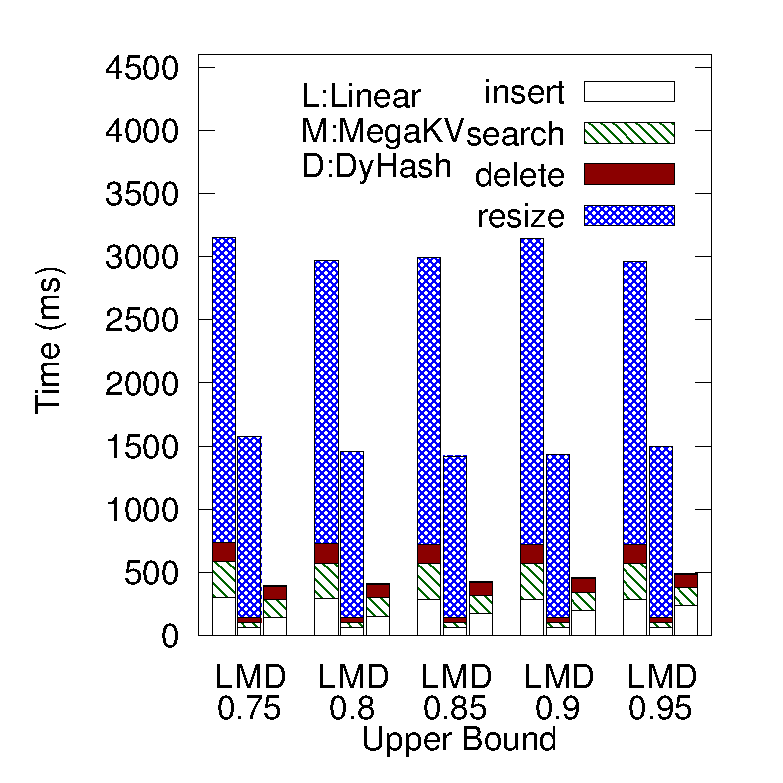
\includegraphics[width=\linewidth]{pic/dynamic/twitter/diff_upper.eps}
		\centerline{\dstwitter}
	\end{minipage}
	\begin{minipage}{0.19\linewidth}\centering
		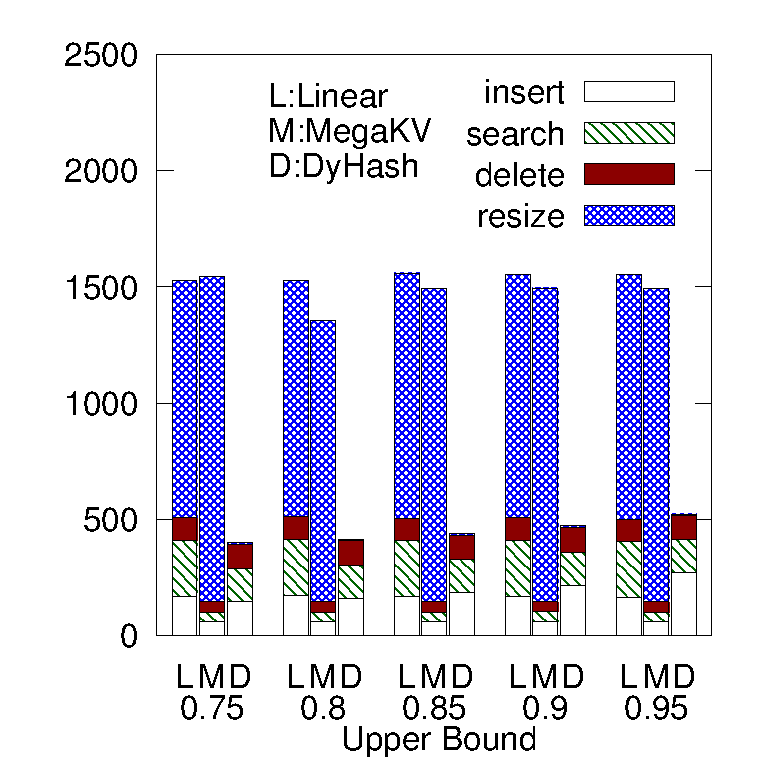
\includegraphics[width=\linewidth]{pic/dynamic/reddit/diff_upper.eps}
		\centerline{\dsreddit}
	\end{minipage}
	\begin{minipage}{0.19\linewidth}\centering
		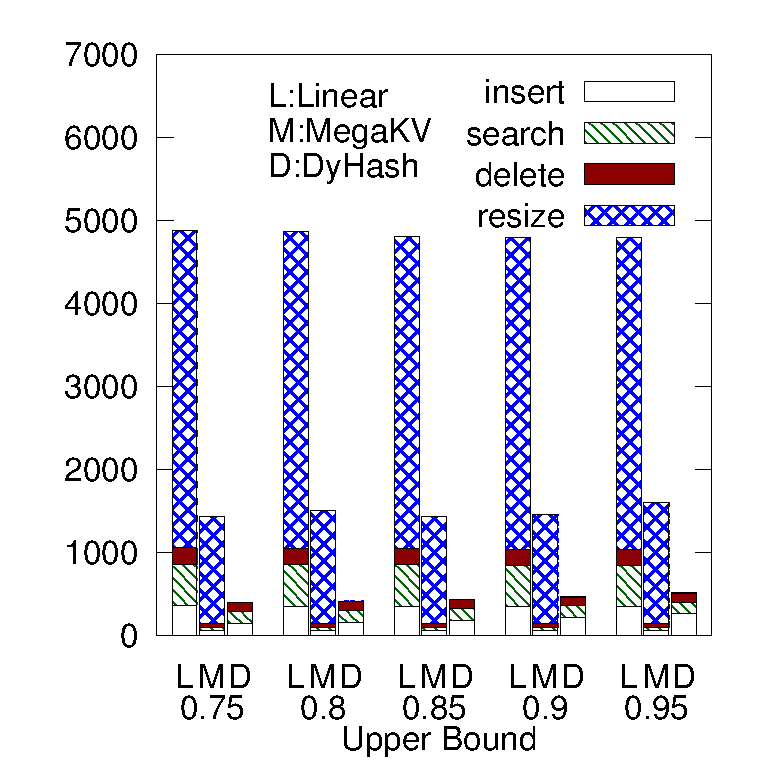
\includegraphics[width=\linewidth]{pic/dynamic/tpch/diff_upper.eps}
		\centerline{\dstpch}
	\end{minipage}
	\begin{minipage}{0.19\linewidth}\centering
		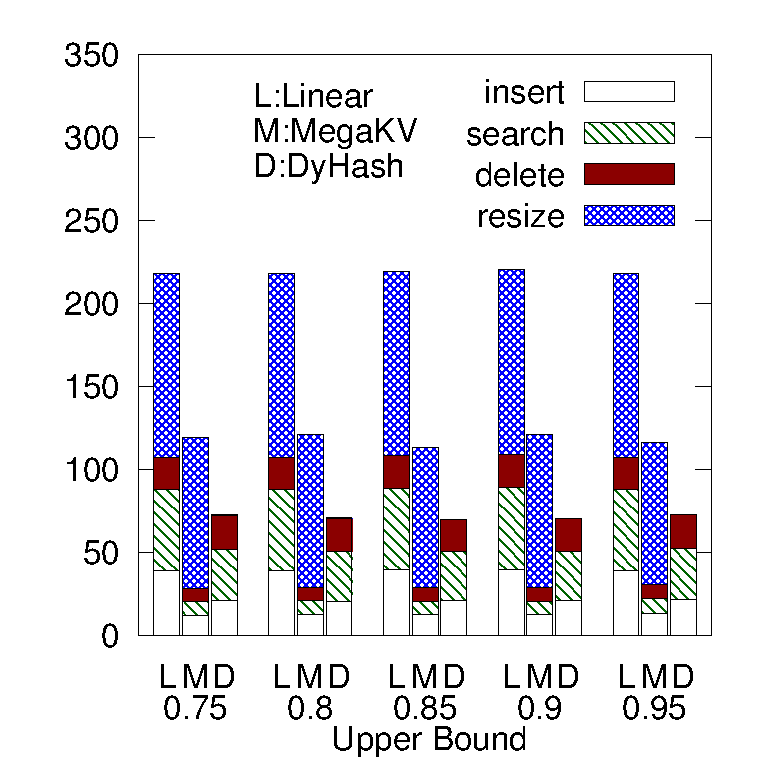
\includegraphics[width=\linewidth]{pic/dynamic/ali/diff_upper.eps}
		\centerline{\dsali}
	\end{minipage}
	\begin{minipage}{0.19\linewidth}\centering
		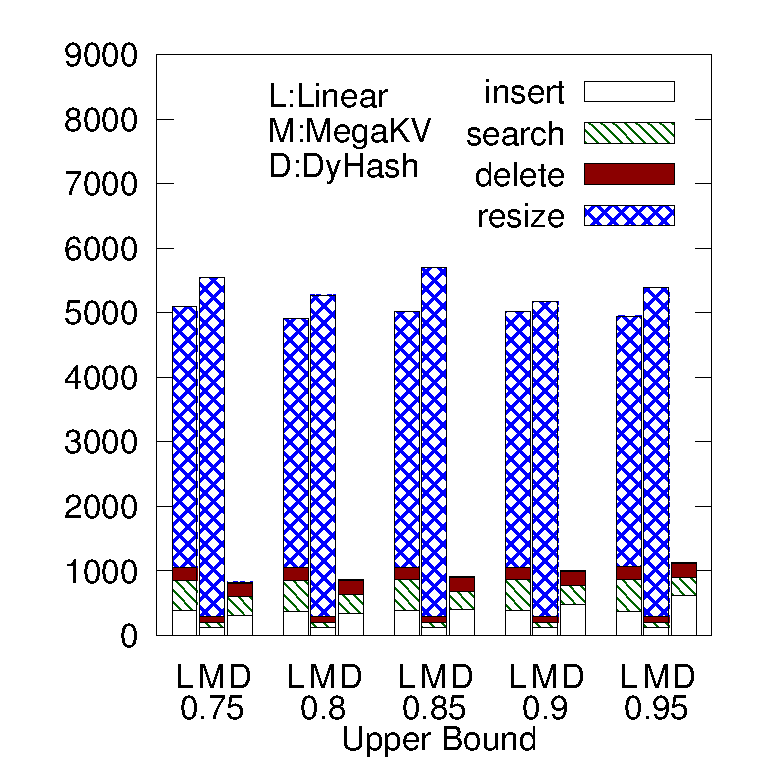
\includegraphics[width=\linewidth]{pic/dynamic/random/diff_upper.eps}
		\centerline{\dsrandom}
	\end{minipage}
	\caption{Run time for varying $\beta$.}
	\label{fig:vary-beta}
\end{figure*}
\begin{figure*}[htp]
	\begin{minipage}{0.19\linewidth}\centering
		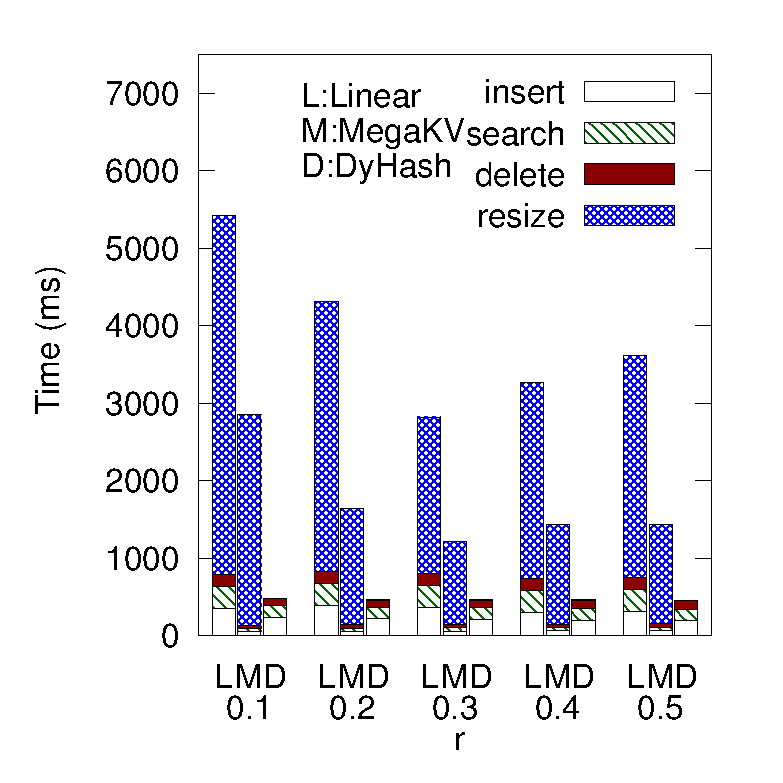
\includegraphics[width=\linewidth]{pic/dynamic/twitter/diff_r.eps}
		\centerline{\dstwitter}
	\end{minipage}
	\begin{minipage}{0.19\linewidth}\centering
		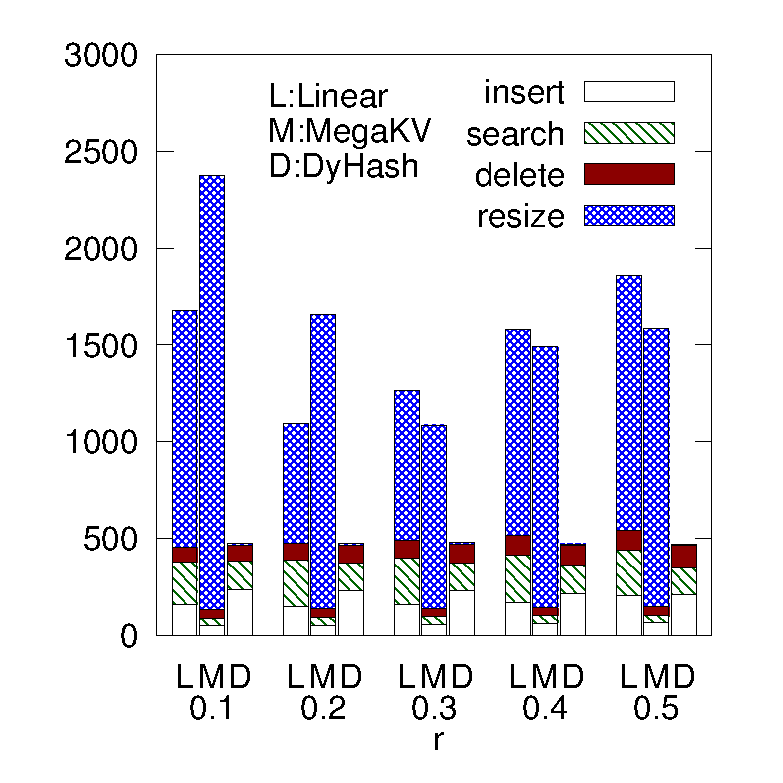
\includegraphics[width=\linewidth]{pic/dynamic/reddit/diff_r.eps}
		\centerline{\dsreddit}
	\end{minipage}
	\begin{minipage}{0.19\linewidth}\centering
		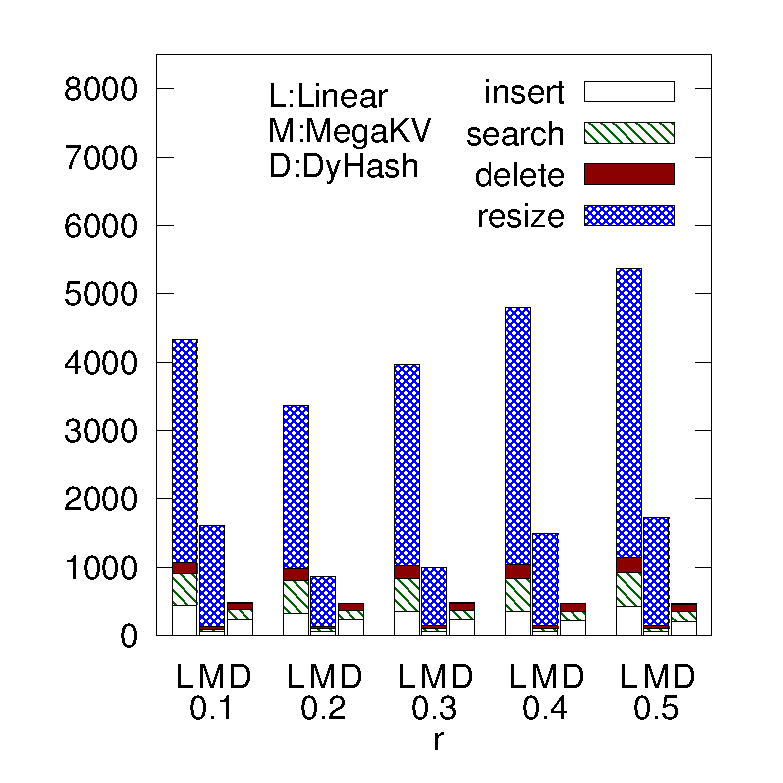
\includegraphics[width=\linewidth]{pic/dynamic/tpch/diff_r.eps}
		\centerline{\dstpch}
	\end{minipage}
	\begin{minipage}{0.19\linewidth}\centering
		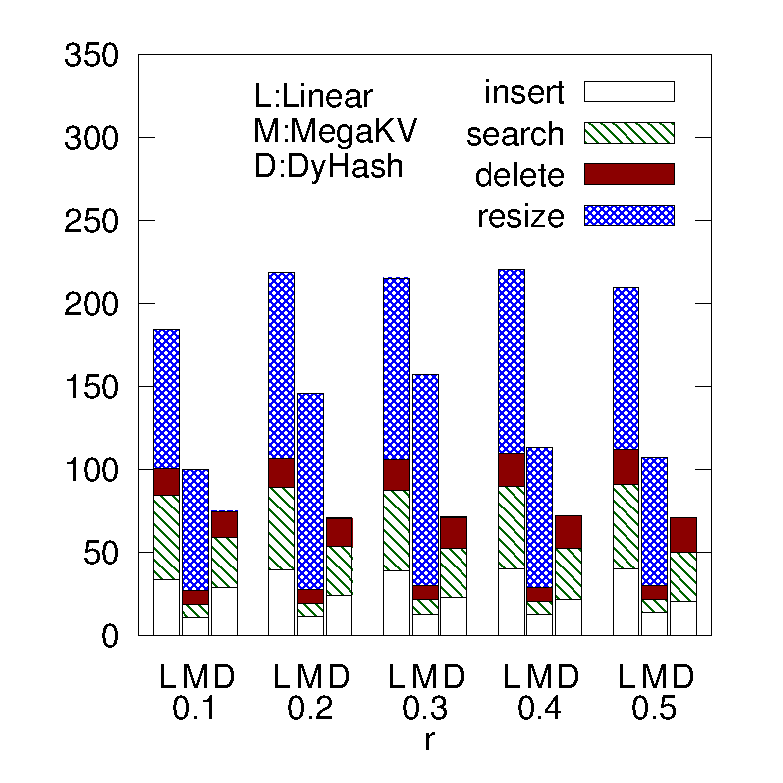
\includegraphics[width=\linewidth]{pic/dynamic/ali/diff_r.eps}
		\centerline{\dsali}
	\end{minipage}
	\begin{minipage}{0.19\linewidth}\centering
		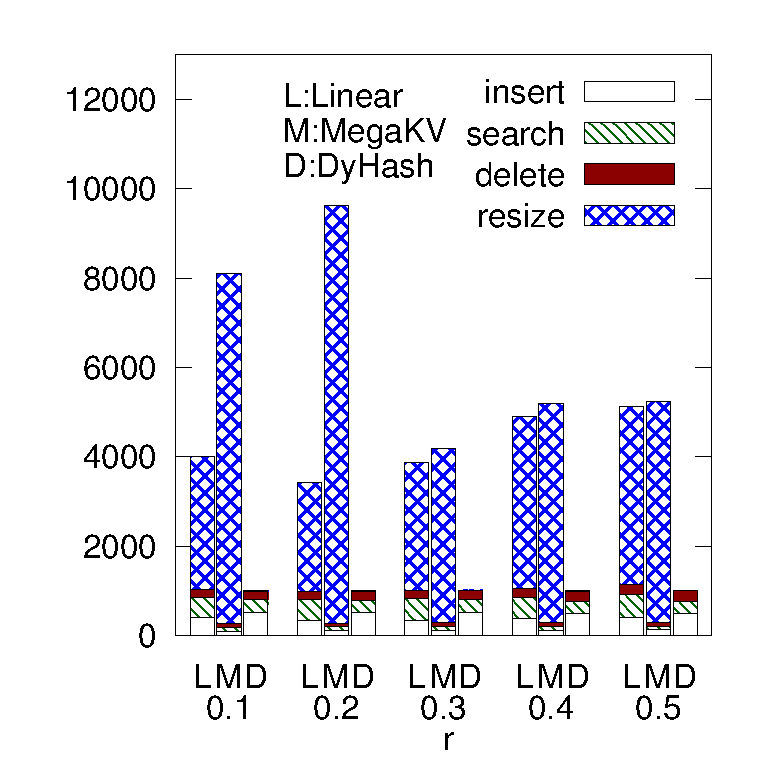
\includegraphics[width=\linewidth]{pic/dynamic/random/diff_r.eps}
		\centerline{\dsrandom}
	\end{minipage}
	\caption{Run time for varying $r$.}
	\label{fig:vary-r-time}
\end{figure*}

\begin{figure*}[ht]
	\begin{minipage}{0.19\linewidth}\centering
		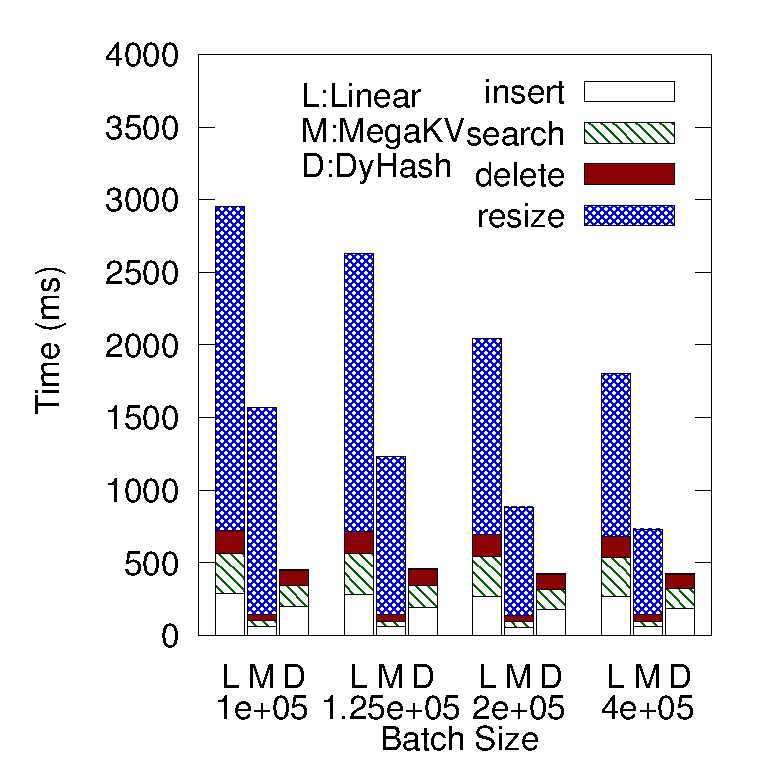
\includegraphics[width=\linewidth]{pic/dynamic/twitter/diff_batch_size.eps}
		\centerline{\dstwitter}
	\end{minipage}
	\begin{minipage}{0.19\linewidth}\centering
		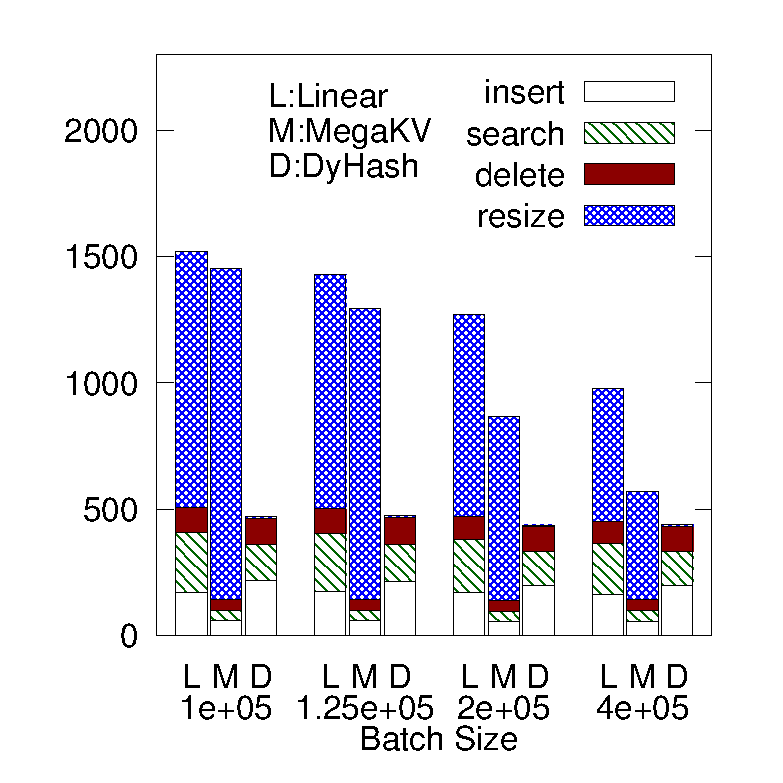
\includegraphics[width=\linewidth]{pic/dynamic/reddit/diff_batch_size.eps}
		\centerline{\dsreddit}
	\end{minipage}
	\begin{minipage}{0.19\linewidth}\centering
		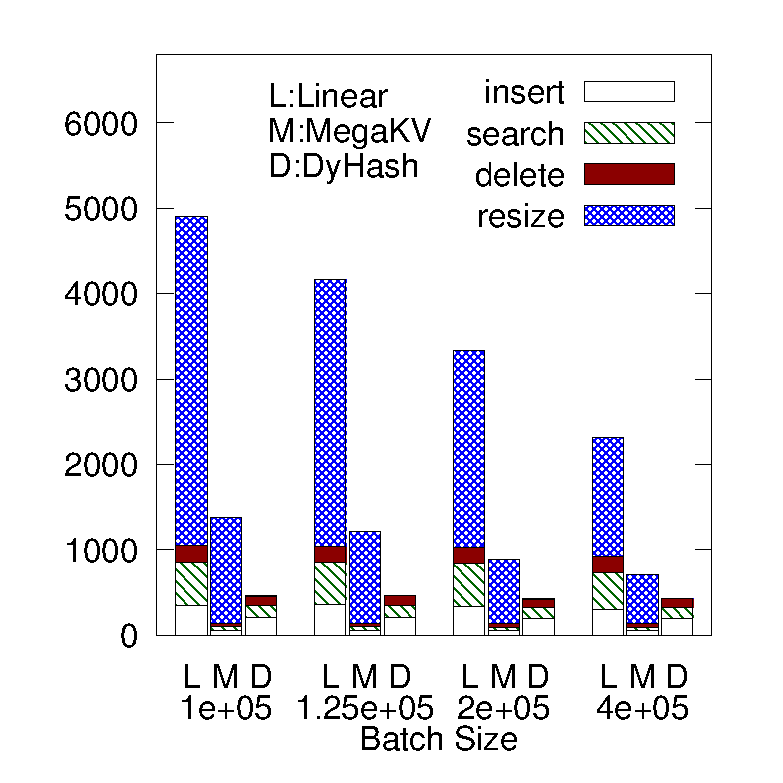
\includegraphics[width=\linewidth]{pic/dynamic/tpch/diff_batch_size.eps}
		\centerline{\dstpch}
	\end{minipage}
	\begin{minipage}{0.19\linewidth}\centering
		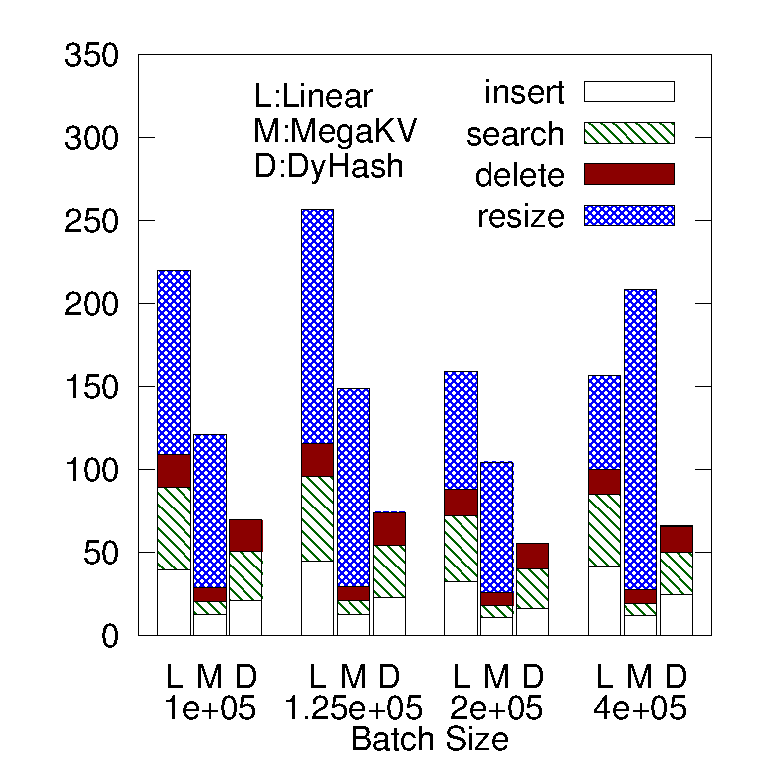
\includegraphics[width=\linewidth]{pic/dynamic/ali/diff_batch_size.eps}
		\centerline{\dsali}
	\end{minipage}
	\begin{minipage}{0.19\linewidth}\centering
		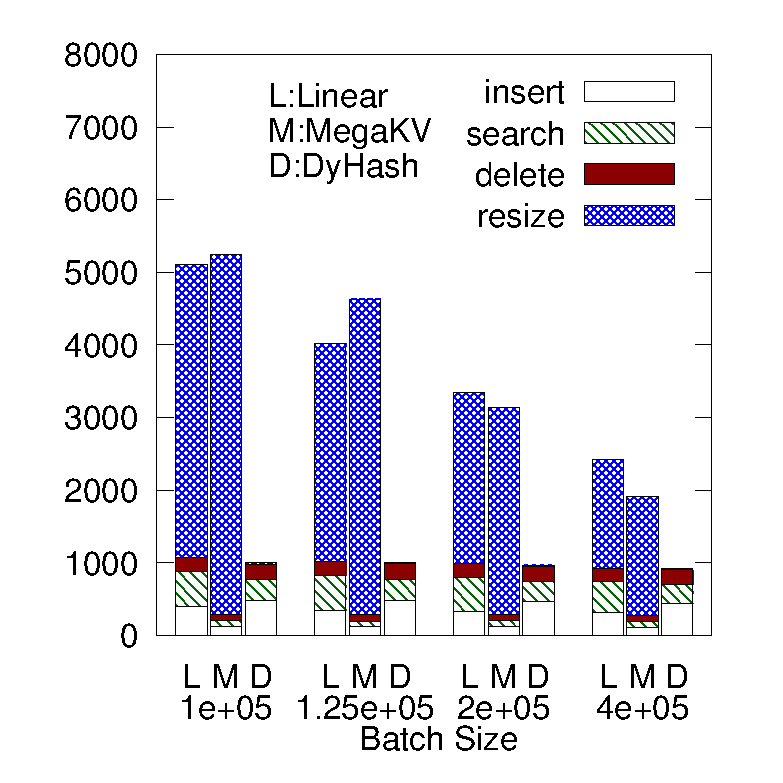
\includegraphics[width=\linewidth]{pic/dynamic/random/diff_batch_size.eps}
		\centerline{\dsrandom}
	\end{minipage}
	\caption{Run time for varying the batch size.}
	\label{fig:vary-batch-size}
\end{figure*}


\begin{figure*}[ht]
	\begin{minipage}{0.19\linewidth}\centering
		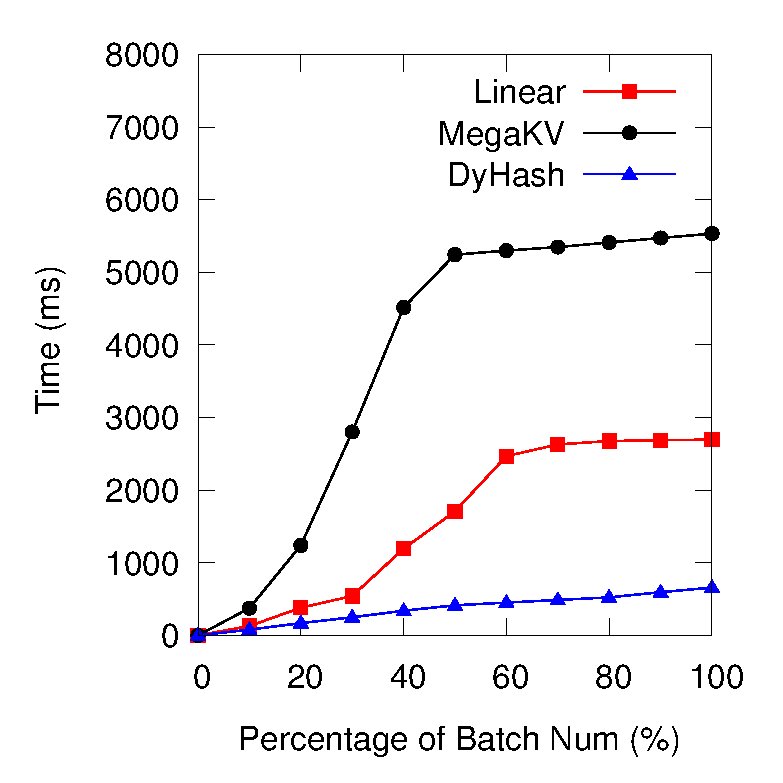
\includegraphics[width=\linewidth]{pic/dynamic-stability/dynamic-sta-twitter.eps}
		\centerline{\dstwitter}
	\end{minipage}
	\begin{minipage}{0.19\linewidth}\centering
		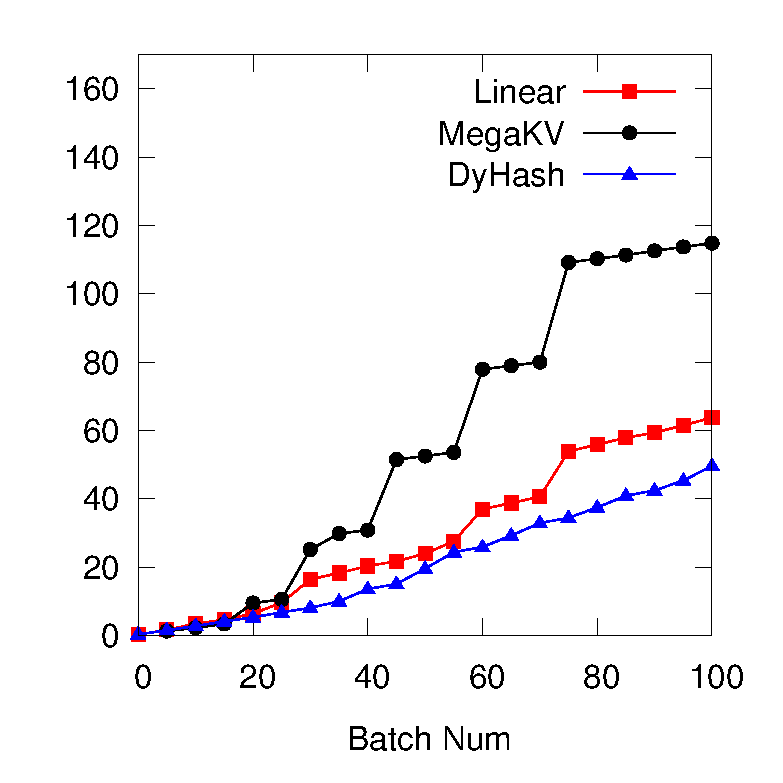
\includegraphics[width=\linewidth]{pic/dynamic-stability/dynamic-sta-reddit.eps}
		\centerline{\dsreddit}
	\end{minipage}
	\begin{minipage}{0.19\linewidth}\centering
		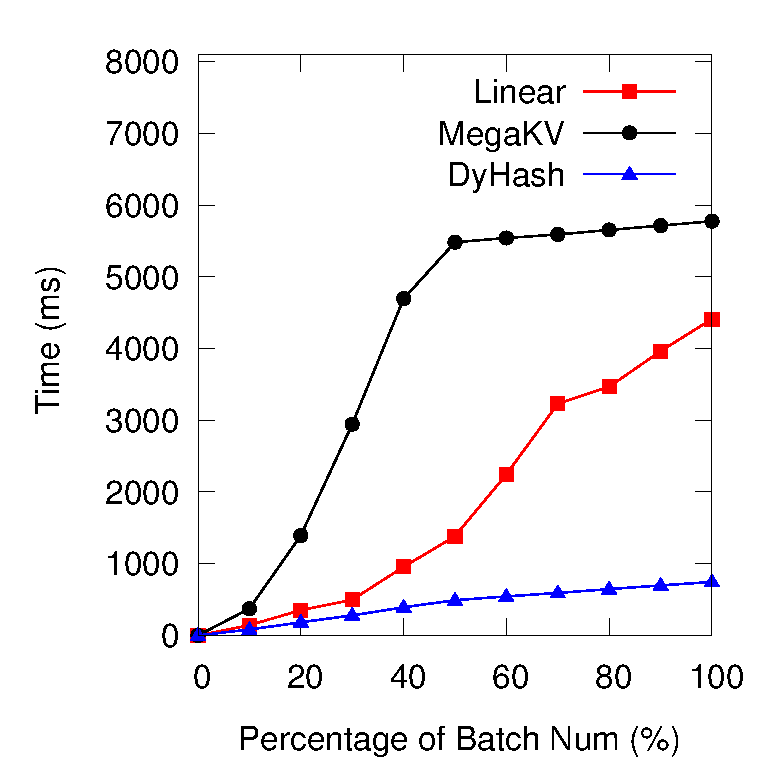
\includegraphics[width=\linewidth]{pic/dynamic-stability/dynamic-sta-tpch.eps}
		\centerline{\dstpch}
	\end{minipage}
	\begin{minipage}{0.19\linewidth}\centering
		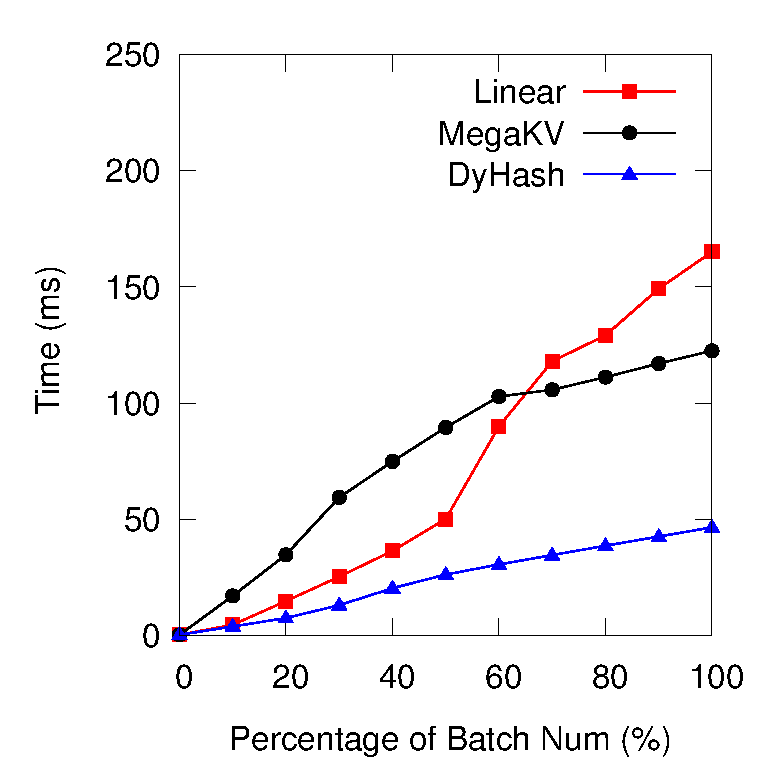
\includegraphics[width=\linewidth]{pic/dynamic-stability/dynamic-sta-ali.eps}
		\centerline{\dsali}
	\end{minipage}
	\begin{minipage}{0.19\linewidth}\centering
		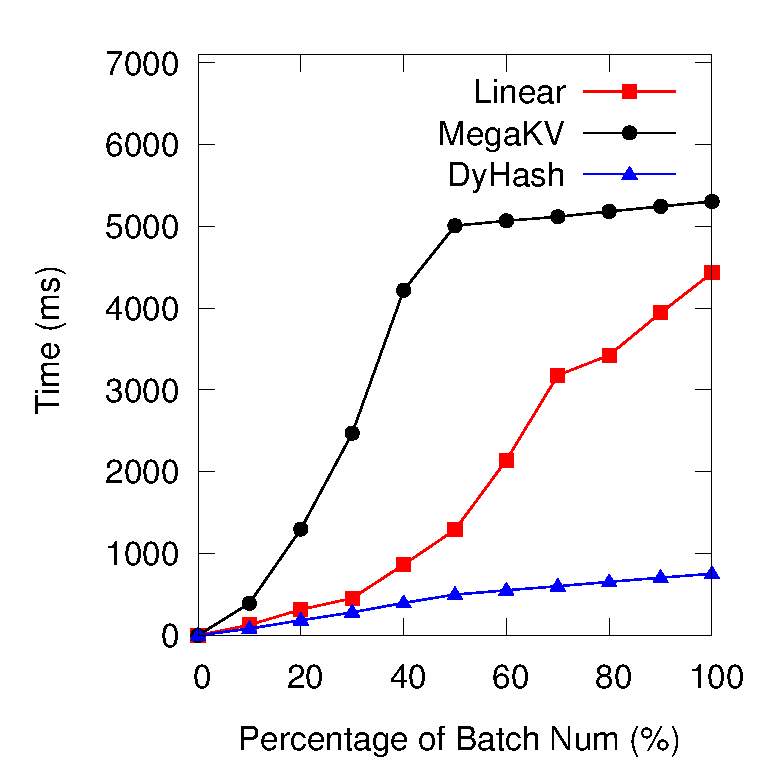
\includegraphics[width=\linewidth]{pic/dynamic-stability/dynamic-sta-random.eps}
		\centerline{\dsrandom}
	\end{minipage}
	\caption{System stability.}
	\label{fig:stability}
\end{figure*}


\subsection{Static Hashing Comparison}\label{sec:exp:static}

\vspace{1mm}\noindent\textbf{Throughput Analysis.} We present the throughput of all compared approaches in Figure~\ref{fig:static} when varying the filled factor. 
First of all, GPU-based approaches are orders of magnitude faster than \google (2  million ops for \formal{insert} and 6 million ops for \formal{find} on average), which validates the motivation of designing hash tables on GPUs. 
Among GPU hash tables, \megakv delivers the best performance across all datasets except for \dsali. Nevertheless, for \formal{insert}, the drawback of \megakv is that it fails to insert some of the KV pairs. Tables~\ref{tab:fail:tw}-\ref{tab:fail:com} present the percentages of insertion failure for varying filled factor across all datasets. \megakv has up to 2.5\% failure rate for the default filled factor, which is the highest among all approaches. 
Our proposed \voter has near-zero failure rate and achieves the 2nd best performance behind \megakv. We note that \cudpp obtains a significant advantage over all approaches in the \dsali dataset. This is because \cudpp will immediately terminate its GPU kernel once it finds some KV pairs cannot be inserted after a number of lookups. This explains why \cudpp has a superior performance since it early terminates on \dsali due to failed insertions (Table~\ref{tab:fail:com}). For \formal{find}, \megakv achieves the best performance as it only has two hash functions. This explains why \voter is slower since we use three hash tables and additional IO lookups are required for each \formal{find}. Both \megakv and \voter are faster than \cudpp and \linear since they employs the bucket mechanism for storing multiple KV pairs contiguously under the same hash value, which exhibits better coalesced memory access.  




For interested readers, please find the throughput results for varying the filled factor across all datasets in the appendix (Figure~\ref{fig:static:all:insert} and~\ref{fig:static:all:search}). 





\vspace{1mm}\noindent\textbf{GPU Profiling.} To further study the behavior of the approaches, we present three types of profiling results for all \formal{insert} GPU kernels in Figure~\ref{fig:static:profile}.
For \emph{warp efficiency}, \voter maintains a stable rate at around 70\%, which is significantly higher than the other two cuckoo hash approaches: \megakv and \cudpp.  
We attribute this phenomenon to the voter mechanism proposed in Section~\ref{sec:vot:con}, which yields better overall load balancing. 
\linear could achieve higher warp efficiency than \voter, but is very volatile across different datasets. This is because each \formal{insert} in \linear may require scanning varying number of hash values for distinct data distributions. 
For example, in the \dsali dataset, its warp efficiency drops below 40\% since \dsali contains more duplicated keys than other datasets. 

Looking at \emph{cache} and \emph{memory bandwidth} profiling results, \megakv and \voter demonstrate better utilization as they employ the bucket mechanism.
As \voter always needs to use atomicCAS to lock a bucket before accessing it, its utilization is inferior than that of \megakv due to the additional IO when inserting a KV pair to a bucket. In addition, atomicCAS is less efficient than atomicExch as it involves more workload per operation (see Table~\ref{fig:atomic}). Nevertheless, implementations based on atomicExch only supports KV pair with 64 bits, whereas adopting atomicCAS in \voter can support arbitrary length as we lock the bucket for exclusive update.
It is also noted that, even though \megakv has great cache utilization due to the use of atomicExch accessing buckets directly, the overall performance is eventually bounded by device memory IOs. 

In summary, under the static environment, \voter achieves competitive efficiency against the compared GPU baselines. Moreover, although \voter does not deliver the best performance over existing approaches, it has very low insertion failure rate and supports more general hash tables.






\subsection{Dynamic Hashing Comparison}\label{sec:exp:dynamic}

\vspace{1mm}\noindent\textbf{Varying the filled factor lower bound $\alpha$.}
We vary the lower bound of the filled factor and report the results in Figure~\ref{fig:vary-alpha-time}. 
The performance is measured by the total running time for processing all batches described in Section~\ref{sec:exp:setup}. Furthermore, we indicate the time taken for all components involved in the processing: \formal{insert}, \formal{find}, \formal{delete} and \formal{resize}. Apparently, the resizing strategy adopted by \linear and \megakv incur significant overhead. Such an overhead grows dramatically for a higher $\alpha$ since more downsizing is required. It is noted that the impact of resizing is the more significant for \megakv than \linear. We interpret the phenomenon as the following.
\megakv has a higher insertion failure rate than that of \linear (see Table~\ref{tab:fail:tw}-\ref{tab:fail:com}). Thus \megakv triggers more upsizing operations leading to a lower filled ratio when resized. As each processing batch contains deletions, \megakv is prone to downsizing when the filled factor falls below $\alpha$ after deletions materialize.
The overhead of repeated upsizing and downsizing severely degrades the performance of \megakv, for the major reason of maintaining the filled factor above $\alpha$. 
The only exception is where $\alpha$ is very small (i.e., $\alpha=0.25$) and \megakv does not need to perform downsize regularly. However, small $\alpha$ means the hash table is mostly empty and thus wastes GPU memory resources.
In contrast, \voter achieves significant speedups over \linear and \megakv (up to \xxx and \xxx faster respectively under the default setting). 
\voter can support even larger $\alpha$ (i.e., $\beta\cdot\frac{d}{d+1}$) but we omit the results since the baselines cannot deliver reasonable performance beyond $\alpha > 0.5$.
There are two reasons behind why \voter's performance. First, \voter has very low failure rate and thus avoids unnecessary upsizing and downsizing operations. Second, \voter employs the resizing strategy (proposed in Section~\ref{sec:dyn}) by only relocating the entries in one subtable efficiently. 
Compared with time taken by \formal{insert}, \formal{delete} and \formal{find}, the cost of \formal{resize} for \voter is almost negligible as shown by the results. 



\vspace{1mm}\noindent\textbf{Varying the filled factor upper bound $\beta$.}
The results for varying $\beta$ is reported in Figure~\ref{fig:vary-beta}. 
It is interesting to see that the upper bound does not significantly affect the overall performance for all methods. 
For \linear and \megakv, it is very hard for them to achieve high filled factor since upsizing will be triggered once there are failed insertions.
Although \voter also incurs cases for failed insertions. Nevertheless, such cases only occur for filled factor beyond $0.9$ and the resizing operations are rarely invoked for the sake of handling failed insertions. 
For \voter, there is a slight increasing trend for a larger $\beta$, especially in the \dsreddit and the \dsrandom datasets. 
The increase is mostly attributed to the additional processing workload of the insertions at a higher filled factor, rather than the resizing cost. 



\vspace{1mm}\noindent\textbf{Varying insert vs. delete ratio $r$.}
In Figure~\ref{fig:vary-r-time}, we report the results for varying the ratio $r$. \linear and \megakv remains inefficient as they incur expensive overheads of resizing. An interesting observation for \linear and \megakv is that there exists some sweet spots where the resizing cost is the minimal.
It is because the workload composition of insertions and deletions should be just right so that it does not trigger unnecessary upsizing or downsizing. However, in reality, the workloads could vary significantly and existing methods cannot be easily adapted while maintaining guaranteed filled factor. This has again validated the effectiveness of \voter against dynamic workloads.



\vspace{1mm}\noindent\textbf{Varying the batch size.}
We have also varied the size of each processing batch. The results are reported in Figure~\ref{fig:vary-batch-size}. \voter remains the most efficient method over \linear and \megakv. It is not surprised to find that the performance of \linear and \megakv is the worst for the smallest batch size, since a fine grained processing batch triggers additional resizing for \linear and \megakv. 



\vspace{1mm}\noindent\textbf{System stability.}
To test the system stability, we track the elapsed time for processing the first 100 batches and report the results in Figure~\ref{fig:stability}. The trend shows that \linear and \megakv incur performance bumps for a number of locations. This is mainly triggered by the resizing operations to handle failed insertions, which also explains the effect is more evident on \megakv than that on \linear. For \voter, the elapsed time shows a smooth trend which indicate the resizing operation does not have visible impact on the performance. 


